% Unified market analysis for semi-humanoid robotics and its software stack
\documentclass[11pt,a4paper]{article}

\usepackage[margin=2.15cm]{geometry}
\usepackage[T1]{fontenc}
\usepackage[utf8]{inputenc}
\usepackage{lmodern}
\usepackage{microtype}
\usepackage{xcolor}
\usepackage{booktabs,tabularx,array}
\usepackage{amsmath,amssymb}
\usepackage{enumitem}
\usepackage{tikz}
\usetikzlibrary{arrows.meta,positioning,shapes.geometric,fit,calc,backgrounds}
\usepackage{hyperref}
\hypersetup{colorlinks=true,linkcolor=navy,urlcolor=navy,citecolor=navy,pdftitle={Semi-Humanoid Robotics: Unified Market Analysis}}
\definecolor{navy}{HTML}{123047}
\definecolor{teal}{HTML}{007C7A}
\definecolor{sky}{HTML}{DCEFF1}
\definecolor{orange}{HTML}{E67E22}
\definecolor{lightgray}{HTML}{F3F6F7}
\setlength{\parskip}{0.45em}
\setlength{\parindent}{0pt}
\renewcommand{\arraystretch}{1.18}
\newcommand{\source}[1]{\par\vspace{-0.25em}\footnotesize\color{gray}\emph{Source: #1}\normalsize}
\newcolumntype{Y}{>{\raggedright\arraybackslash}X}

\begin{document}

\begin{titlepage}
\color{navy}
\vspace*{1.4cm}
{\Large MARKET INTELLIGENCE REPORT\par}
\vspace{0.4cm}
{\huge\bfseries Semi-Humanoid Robotics\par}
\vspace{0.15cm}
{\Large\bfseries Unified Market Analysis: Hardware, High-Level Software and Real-Time Control\par}
\vspace{1.1cm}
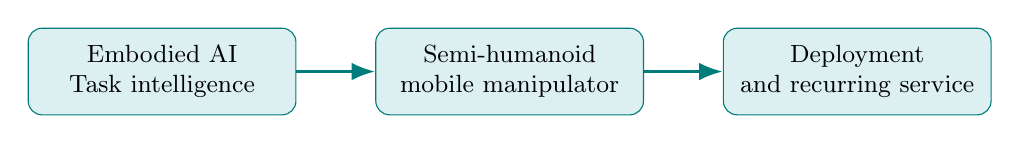
\begin{tikzpicture}[every node/.style={font=\small}]
  \node[draw=teal,fill=sky,rounded corners=5pt,minimum width=3.4cm,minimum height=1.1cm,align=center] (ai) {Embodied AI\\Task intelligence};
  \node[draw=teal,fill=sky,rounded corners=5pt,minimum width=3.4cm,minimum height=1.1cm,right=1.0cm of ai,align=center] (robot) {Semi-humanoid\\mobile manipulator};
  \node[draw=teal,fill=sky,rounded corners=5pt,minimum width=3.4cm,minimum height=1.1cm,right=1.0cm of robot,align=center] (ops) {Deployment\\and recurring service};
  \draw[-{Latex[length=3mm]},very thick,teal] (ai)--(robot);
  \draw[-{Latex[length=3mm]},very thick,teal] (robot)--(ops);
\end{tikzpicture}
\vfill
\begin{tabular}{@{}ll@{}}
\textbf{Purpose} & Investment, product and go-to-market decision support \\
\textbf{Scope} & Wheeled semi-humanoids / autonomous mobile manipulators; software from cloud to firmware \\
\textbf{Prepared} & August 2026 \\
\textbf{Evidence base} & Supplied market-analysis dossiers and cited primary/vendor/market sources \\
\end{tabular}
\vspace{1.2cm}
\end{titlepage}

\tableofcontents
\newpage

\section{Executive view}

\textbf{Investment thesis.} Semi-humanoid robotics is best understood as the commercially pragmatic intersection of an autonomous mobile robot (AMR), a collaborative manipulator, and an embodied-AI data platform. A wheeled base avoids the energy, fall-risk and whole-body-control burden of bipedal locomotion while bimanual upper-body kinematics preserve human-environment reach and interaction. The category is therefore positioned to automate material movement plus the manipulation steps that historically required people.

\textbf{Market signal.} Published estimates are not directly comparable because they draw different boundaries around AMRs, mobile manipulators, service robots, systems integration and software. The narrowest supplied estimate, autonomous mobile manipulator robots (AMMRs), grows from \$385.9m in 2023 to \$1.699bn in 2030 (23.9\% CAGR). A focused mobile-manipulator estimate reaches \$3.95bn in 2032 from \$1.52bn in 2025 (14.7\% CAGR). These figures support a strong-growth conclusion, but \emph{must be used as scenario anchors rather than summed into one market size}.\cite{gvr,mnm}

\textbf{Strategic implication.} The defensible product wedge is not ``general humanoid.'' It is a repeatable, bounded workflow with measurable throughput and low commissioning friction: intralogistics line-feeding, laboratory material handling, or light industrial kitting. Differentiation should compound across three layers: safe, serviceable hardware; reliable autonomy; and a data/operations layer that improves deployed fleets.

\begin{center}
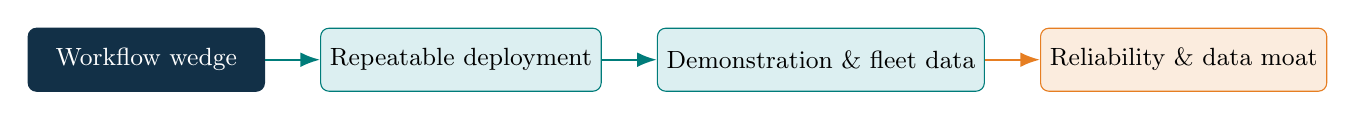
\begin{tikzpicture}[node distance=0.55cm and 0.7cm, every node/.style={font=\small,align=center}]
\node[draw=navy,fill=navy,text=white,rounded corners=3pt,minimum width=3.0cm,minimum height=0.8cm] (wedge) {Workflow wedge};
\node[draw=teal,fill=sky,rounded corners=3pt,minimum width=3.0cm,minimum height=0.8cm,right=of wedge] (repeat) {Repeatable deployment};
\node[draw=teal,fill=sky,rounded corners=3pt,minimum width=3.0cm,minimum height=0.8cm,right=of repeat] (data) {Demonstration \& fleet data};
\node[draw=orange,fill=orange!15,rounded corners=3pt,minimum width=3.0cm,minimum height=0.8cm,right=of data] (moat) {Reliability \& data moat};
\draw[-{Latex[length=2.5mm]},thick,teal] (wedge)--(repeat);
\draw[-{Latex[length=2.5mm]},thick,teal] (repeat)--(data);
\draw[-{Latex[length=2.5mm]},thick,orange] (data)--(moat);
\end{tikzpicture}
\end{center}

\section{Category definition and strategic boundaries}

This report uses \textbf{semi-humanoid} to mean a wheeled mobile manipulator with an anthropomorphic upper body---typically one or two articulated arms, a perception head and compliant end effectors. It includes AMMRs and research/service mobile manipulators where the system can navigate and manipulate. It excludes stationary cobots, pure AMRs and full bipedal humanoids unless used as a reference class.

\begin{figure}[ht]
\centering
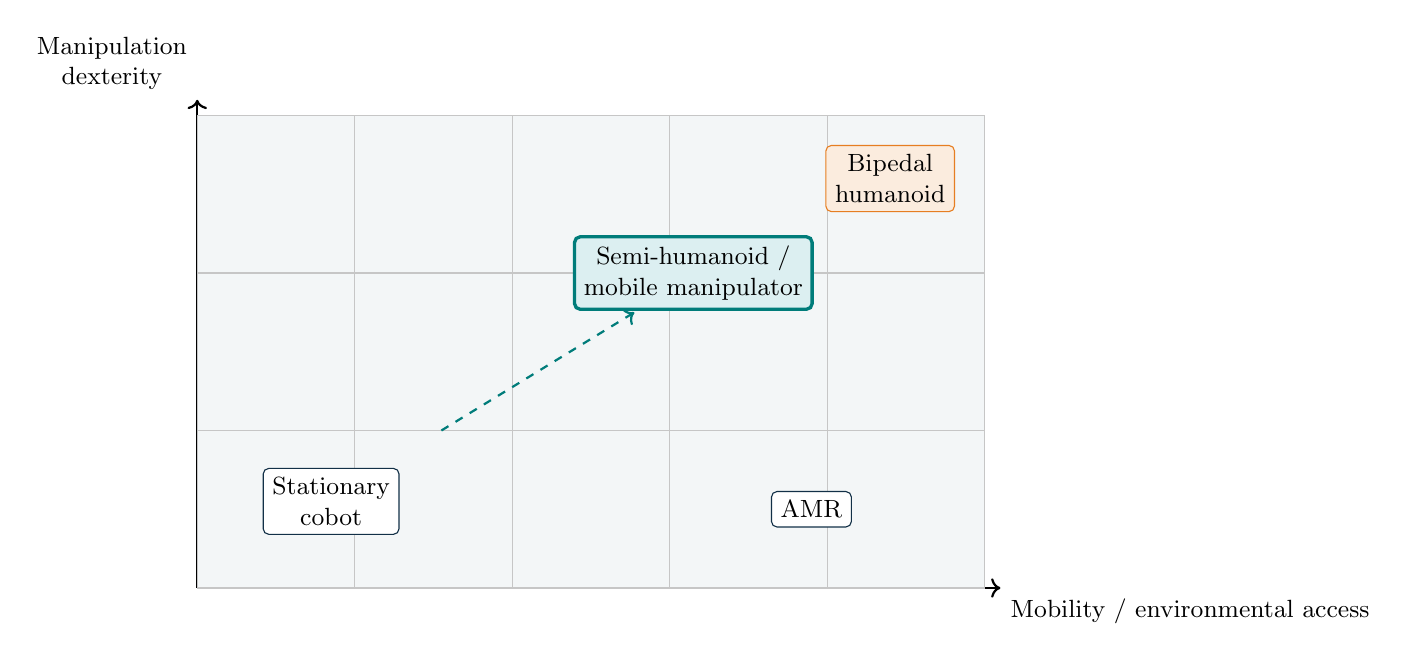
\begin{tikzpicture}[x=1cm,y=1cm,font=\small]
  \draw[->,thick] (0,0)--(10.2,0) node[below right]{Mobility / environmental access};
  \draw[->,thick] (0,0)--(0,6.2) node[above left,align=center]{Manipulation\\dexterity};
  \fill[lightgray] (0,0) rectangle (10,6);
  \draw[step=2cm,gray!45] (0,0) grid (10,6);
  \node[draw=navy,fill=white,rounded corners=2pt,align=center] at (1.7,1.1) {Stationary\\cobot};
  \node[draw=navy,fill=white,rounded corners=2pt,align=center] at (7.8,1.0) {AMR};
  \node[draw=teal,fill=sky,very thick,rounded corners=2pt,align=center] at (6.3,4.0) {Semi-humanoid /\\mobile manipulator};
  \node[draw=orange,fill=orange!15,rounded corners=2pt,align=center] at (8.8,5.2) {Bipedal\\humanoid};
  \draw[->,dashed,thick,teal] (3.1,2.0)--(5.55,3.5);
\end{tikzpicture}
\caption{Category positioning: semi-humanoids target the high-value overlap of mobility and dexterous manipulation without requiring bipedal locomotion.}
\label{fig:positioning}
\end{figure}

\subsection{Why the wheeled form factor matters}

For a static support polygon $\mathcal{P}$, a basic feasibility condition is that the ground projection of the system centre of mass remains inside the polygon:
\begin{equation}
 \Pi_{xy}\!\left(\mathbf{r}_{\mathrm{CoM}}\right) \in \mathcal{P}, \qquad
 \mathbf{r}_{\mathrm{CoM}}(\mathbf{q})=\frac{m_b\mathbf{r}_b+m_t\mathbf{r}_t+\sum_{i=1}^{n}m_i\mathbf{r}_i(\mathbf{q})}{m_b+m_t+\sum_{i=1}^{n}m_i}.
\end{equation}
For a wheeled platform, this constraint can be managed through footprint, mass distribution, arm acceleration limits and payload envelopes. A biped must additionally sustain dynamically stable gait and fall recovery. This does not make wheels universally better---stairs remain a clear limitation---but it improves readiness for flat-floor industrial and institutional environments.

\begin{table}[ht]
\centering\small
\caption{Form-factor trade-off relevant to near-term deployments.}
\begin{tabularx}{\textwidth}{@{}lYY@{}}
\toprule
Dimension & Wheeled semi-humanoid & Bipedal humanoid \\
\midrule
Continuous runtime & Typically up to an 8-hour shift-class target in benchmark platforms & Often constrained by dynamic locomotion energy demand \\
Control burden & Navigation plus manipulation; stable base simplifies planning & Whole-body gait, balance and fall recovery \\
Facility access & Excellent on flat floors, ramps and standard doorways & Potentially superior on stairs and discontinuous terrain \\
Commercial fit today & Bounded industrial, logistics, lab and service workflows & Longer-horizon general access and infrastructure adaptation \\
\bottomrule
\end{tabularx}
\source{Synthesis of supplied analyses; platform examples from \cite{stretchpaper,reachy}.}
\end{table}

\section{Market opportunity: size, growth and adoption}

\subsection{A range-based market model}

Market research providers employ different units of analysis. The useful reading is a nested set: AMMR is the narrow product category; mobile manipulation is a broader product category; mobile robots includes adjacent vehicle, software and service revenue. Equation~\ref{eq:cagr} provides the consistency check for every published forecast:
\begin{equation}
 \mathrm{CAGR}=\left(\frac{V_T}{V_0}\right)^{\frac{1}{T}}-1.
 \label{eq:cagr}
\end{equation}

\begin{table}[ht]
\centering\small
\caption{Published market anchors---comparable only within their stated scope.}
\begin{tabularx}{\textwidth}{@{}lrrrrY@{}}
\toprule
Scope & Base & Year & Forecast & Year & CAGR / interpretation \\
\midrule
AMMR (narrow) & \$0.386bn & 2023 & \$1.699bn & 2030 & 23.9\%; integrated mobile manipulators \\
Mobile manipulator & \$1.52bn & 2025 & \$3.95bn & 2032 & 14.7\%; focused category estimate \\
Mobile manipulator (broad) & \$0.89bn & 2025 & \$3.74bn & 2034 & 17.3\%; broader report definition \\
Extended mobile manipulator & \$4.70bn & 2025 & \$14.10bn & 2033 & 13.0\%; wider systems boundary \\
AMR baseline & \$3.10bn & 2025 & \$17.00bn & 2035 & 19.5\%; adjacent mobility opportunity \\
Mobile robots total & \$20.79bn & 2025 & \$63.28bn & 2035 & 11.83\%; includes broad systems/services \\
\bottomrule
\end{tabularx}
\source{Supplied market-analysis dossiers, citing \cite{gvr,mnm,bri,htf,gmi,roots}. Currency values are nominal published estimates.}
\end{table}

\begin{figure}[ht]
\centering
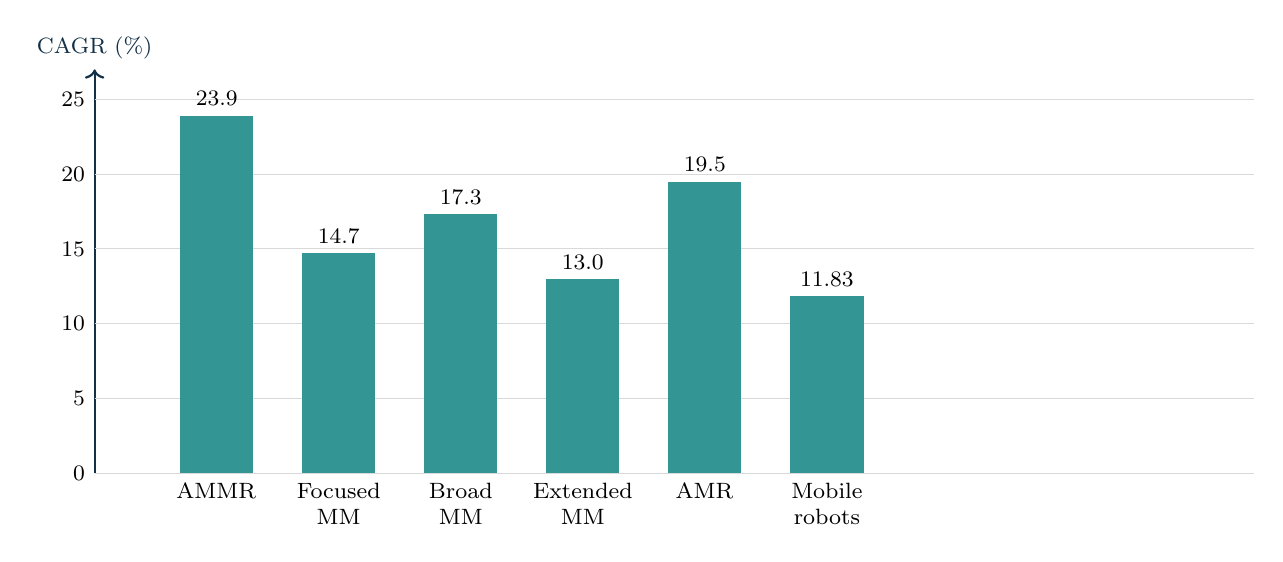
\begin{tikzpicture}[x=1.55cm,y=0.19cm,font=\footnotesize]
  \draw[->,thick,navy] (0,0)--(0,27) node[above]{CAGR (\%)};
  \foreach \y in {0,5,10,15,20,25} {\draw[gray!30] (0,\y)--(9.5,\y); \node[left] at (0,\y) {\y};}
  \foreach \x/\lab/\value in {1/AMMR/23.9,2/Focused MM/14.7,3/Broad MM/17.3,4/Extended MM/13.0,5/AMR/19.5,6/Mobile robots/11.83} {
    \fill[teal!80] (\x-0.3,0) rectangle (\x+0.3,\value);
    \node[above] at (\x,\value) {\value};
    \node[below,align=center,text width=1.35cm] at (\x,0) {\lab};
  }
\end{tikzpicture}
\caption{Growth rates reported across non-identical scopes. The category is attractive; a single ``market size'' is not justified by these sources.}
\label{fig:cagr}
\end{figure}

\subsection{Demand drivers and buying centres}

The primary demand drivers are labour scarcity, throughput pressure in e-commerce and manufacturing, safety/ergonomics, and the need to automate variable tasks without fixed conveyor infrastructure. The first buyers are operations leaders with a quantifiable bottleneck, supported by IT/OT, safety and finance stakeholders. North America is a leading revenue region in the supplied sources, while Asia-Pacific is repeatedly identified as the fastest-growing adoption geography; both signals should be validated per target vertical and country before commercial commitment.\cite{bri,gvr}

\begin{center}

\begin{tikzpicture}[node distance=0.65cm, every node/.style={font=\small,align=center}]
\node[draw=navy,fill=navy,text=white,rounded corners=3pt,minimum width=3.0cm,minimum height=0.7cm] (labor) {Labour / throughput pressure};
\node[draw=teal,fill=sky,rounded corners=3pt,minimum width=3.0cm,minimum height=0.7cm,right=of labor] (case) {Bounded use case};
\node[draw=teal,fill=sky,rounded corners=3pt,minimum width=3.0cm,minimum height=0.7cm,right=of case] (roi) {Measured ROI};
\node[draw=orange,fill=orange!15,rounded corners=3pt,minimum width=3.0cm,minimum height=0.7cm,right=of roi] (scale) {Fleet expansion};
\draw[-{Latex[length=2.5mm]},thick,teal] (labor)--(case);
\draw[-{Latex[length=2.5mm]},thick,teal] (case)--(roi);
\draw[-{Latex[length=2.5mm]},thick,orange] (roi)--(scale);
\end{tikzpicture}
\end{center}

\section{Competitive landscape and product economics}

The market spans three archetypes: low-cost telescoping single-arm systems, bimanual semi-humanoids and heavy industrial mobile manipulators. The strategic gap is a system that makes bimanual or compliant manipulation deployable without importing the cost and commissioning profile of bespoke industrial integration.

\begin{table}[ht]
\centering\small
\caption{Selected benchmark platforms (published specifications; configuration-dependent).}
\begin{tabularx}{\textwidth}{@{}lYrrrY@{}}
\toprule
Platform & Archetype & Price (USD) & Mass & Arm payload & Commercial reading \\
\midrule
Hello Robot Stretch 3/4 & Telescoping single arm & 19,950--29,950 & 46kg & 2.5kg extended & Low-cost, narrow-space mobile manipulation \\
Pollen Reachy 2 & Bimanual semi-humanoid & 70,000--78,000 & 50kg & $\sim$3kg / arm & Data-rich research and HRI platform \\
PAL TIAGo & Industrial/research mobile manipulator & $\sim$56,000--70,000 & 70kg & 3--6kg & Mature ROS ecosystem, configurable \\
Toyota HSR & Service/research mobile manipulator & Proprietary / lease & 37kg & $\sim$1.2kg & Assistive-research benchmark \\
Willow Garage PR2 & Legacy bimanual baseline & $\sim$400,000 & 220kg & $\sim$2kg / arm & Demonstrates historical cost/weight burden \\
\bottomrule
\end{tabularx}
\source{Supplied analyses, citing \cite{stretchpaper,reachy,tiago}. Prices are list/indicative values, not installed-system quotes.}
\end{table}

\subsection{TCO and procurement logic}

The relevant buyer calculation is installed economics, not robot price. A transparent model separates acquisition, integration, operations and residual value:
\begin{equation}
 \mathrm{TCO}_{N}=C_{\mathrm{robot}}+C_{\mathrm{integration}}+\sum_{t=1}^{N}\frac{C_{\mathrm{service},t}+C_{\mathrm{energy},t}+C_{\mathrm{ops},t}}{(1+r)^t}-\frac{V_{\mathrm{residual}}}{(1+r)^N}.
\end{equation}
The investment case becomes positive when discounted labour, throughput, quality and safety benefits exceed $\mathrm{TCO}_{N}$. In practice, integration time, exception handling and uptime dominate the uncertainty. The product roadmap should therefore make site mapping, WMS/ERP connectors, safety validation and recovery behaviours reusable assets.

\section{The software market: where value and defensibility accrue}

Semi-humanoid software is not one market; it is a value chain from embedded control to cloud operations. High-level software converts intent and observations into plans. Low-level software makes physical execution deterministic, safe and observable. The commercial opportunity is recurring when the supplier owns deployment tooling, fleet operations, updates, analytics and workflow integrations---not merely the robot application.

\begin{figure}[ht]
\centering
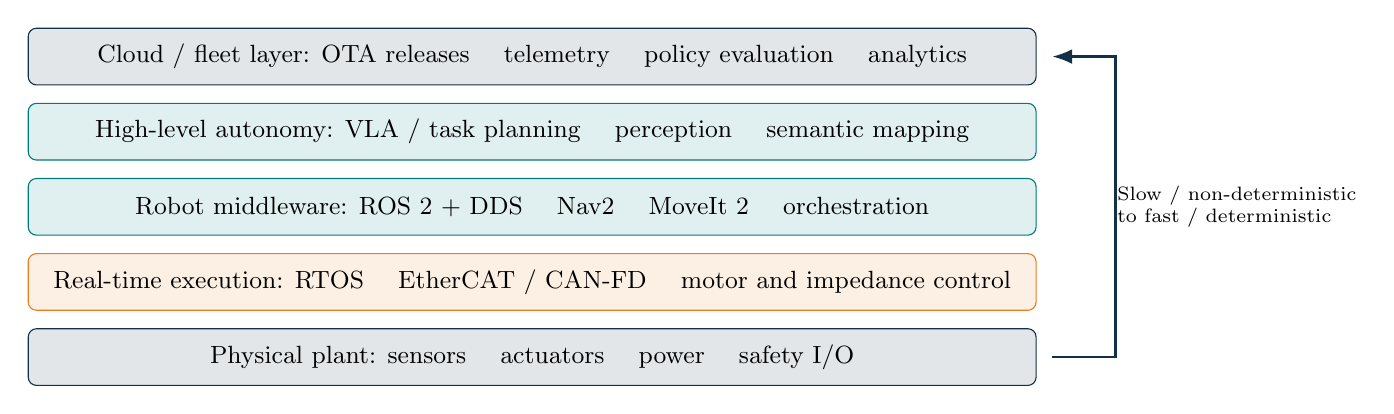
\begin{tikzpicture}[every node/.style={font=\small,align=center},layer/.style={draw=#1,fill=#1!12,rounded corners=3pt,minimum width=12.8cm,minimum height=0.72cm}]
\node[layer=navy] (cloud) {Cloud / fleet layer: OTA releases \quad telemetry \quad policy evaluation \quad analytics};
\node[layer=teal,below=0.22cm of cloud] (cognition) {High-level autonomy: VLA / task planning \quad perception \quad semantic mapping};
\node[layer=teal,below=0.22cm of cognition] (planning) {Robot middleware: ROS~2 + DDS \quad Nav2 \quad MoveIt~2 \quad orchestration};
\node[layer=orange,below=0.22cm of planning] (control) {Real-time execution: RTOS \quad EtherCAT / CAN-FD \quad motor and impedance control};
\node[layer=navy,below=0.22cm of control] (physical) {Physical plant: sensors \quad actuators \quad power \quad safety I/O};
\draw[-{Latex[length=2.5mm]},thick,navy] ($(physical.east)+(0.2,0)$) -- ++(0.8,0) |- ($(cloud.east)+(0.2,0)$);
\node[right=0.9cm of planning,font=\scriptsize,align=left] {Slow / non-deterministic\\to fast / deterministic};
\end{tikzpicture}
\caption{Unified software architecture. Separation of decision-making from real-time safety control is a design requirement, not an implementation preference.}
\label{fig:stack}
\end{figure}

\subsection{High-level software}

At the high level, ROS~2 and DDS provide modular communications; Nav2 handles navigation; MoveIt~2 produces manipulation plans; perception builds scene understanding; and VLA or task models translate human intent into constrained action sequences. Simulation (Isaac Sim/Isaac Lab, MuJoCo and Gazebo) accelerates validation, synthetic data and policy learning.\cite{isaac,isaacsim,mujoco,gazebo}

The attractive software economics lie in workflow packs and operations: site configuration, reusable behaviours, remote diagnostics, secure OTA deployment, teleoperation assistance and fleet analytics. Generic foundation models may lower the cost of cognition, but production-grade reliability, data governance and site integration remain local moats.

\subsection{Low-level software and safety}

Low-level control belongs on deterministic compute, independent of an AI planner. A typical cascade is:
\begin{align}
 \tau_{\mathrm{cmd}} &= K_p(q_d-q)+K_d(\dot q_d-\dot q)+\tau_{\mathrm{ff}},\\
 \mathbf{F}_{\mathrm{cmd}} &= \mathbf{K}(\mathbf{x}_d-\mathbf{x})+\mathbf{D}(\dot{\mathbf{x}}_d-\dot{\mathbf{x}}),
\end{align}
where $q$ is joint state and $\mathbf{x}$ is task-space pose. The firmware enforces torque, velocity, temperature and communication-loss limits before commands reach the actuator. EtherCAT is attractive where high-rate synchronisation is needed; CAN-FD provides a robust, lower-complexity alternative for distributed subsystems.\cite{reachy}

\begin{table}[ht]
\centering\small
\caption{High-level versus low-level software: product and engineering roles.}
\begin{tabularx}{\textwidth}{@{}lYY@{}}
\toprule
Aspect & High-level autonomy & Low-level execution \\
\midrule
Primary goal & Choose and plan useful work & Execute safely and predictably \\
Typical tools & ROS 2, DDS, Nav2, MoveIt 2, VLA/VLM, simulation & RTOS, C/C++/Rust, fieldbus, motor drivers, safety watchdogs \\
Time scale & Tens of milliseconds to seconds & Sub-millisecond to millisecond-class loops \\
Failure posture & Degrade, request help, re-plan & Fail safe, limit energy, maintain deterministic state \\
Commercial lever & Workflow packs, data, fleet operations & Reliability, certification evidence, hardware differentiation \\
\bottomrule
\end{tabularx}
\end{table}

\section{Data flywheel and sim-to-real}

Teleoperation provides an early route to revenue and a disciplined route to autonomy. Demonstrations create labelled observation-action data; simulation expands rare conditions; evaluation gates protect deployment; fleet telemetry identifies exceptions. Domain randomisation varies lighting, textures, friction, mass and latency so policies avoid overfitting to a simulator.\cite{isaacsim,mujoco}

\begin{figure}[ht]
\centering
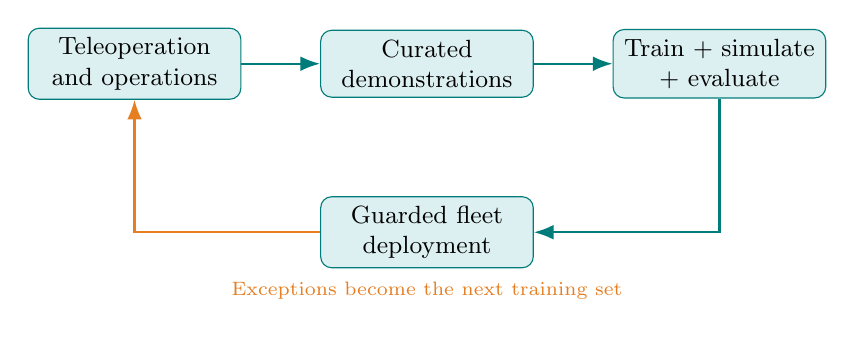
\begin{tikzpicture}[node distance=0.6cm and 1.0cm,every node/.style={font=\small,align=center},box/.style={draw=teal,fill=sky,rounded corners=4pt,minimum width=2.7cm,minimum height=0.85cm}]
\node[box] (teleop) {Teleoperation\\and operations};
\node[box,right=of teleop] (data) {Curated\\demonstrations};
\node[box,right=of data] (train) {Train + simulate\\+ evaluate};
\node[box,below=1.25cm of data] (deploy) {Guarded fleet\\deployment};
\draw[-{Latex[length=2.5mm]},thick,teal] (teleop)--(data);
\draw[-{Latex[length=2.5mm]},thick,teal] (data)--(train);
\draw[-{Latex[length=2.5mm]},thick,teal] (train.south) |- (deploy.east);
\draw[-{Latex[length=2.5mm]},thick,orange] (deploy.west) -| (teleop.south);
\node[below=0.05cm of deploy,font=\scriptsize,text=orange] {Exceptions become the next training set};
\end{tikzpicture}
\caption{A commercial autonomy flywheel: operational data is valuable only when governed, curated and tied to measurable evaluation gates.}
\end{figure}

\section{Go-to-market priorities and risks}

\subsection{Recommended beachheads}

\begin{table}[ht]
\centering\small
\caption{Beachhead screen.}
\begin{tabularx}{\textwidth}{@{}lYYY@{}}
\toprule
Vertical & Initial workflow & Why it fits & Watch-out \\
\midrule
Warehouse / intralogistics & Line feeding, tote movement, simple picking & Clear throughput metrics; flat-floor mobility & WMS integration and exception rate \\
Laboratories / healthcare operations & Specimen, consumable and equipment transport & Repetitive routes; traceability value & Validation, hygiene and liability \\
Electronics / light manufacturing & Kitting, machine tending, material replenishment & High labour value; controlled environments & Precision and cycle-time requirements \\
Research / education & Teleoperation and embodied-AI development & Early-adopter appetite; data creation & Smaller budgets; feature-led buying \\
\bottomrule
\end{tabularx}
\end{table}

\subsection{Risk register and mitigation}

\begin{table}[ht]
\centering\small
\begin{tabularx}{\textwidth}{@{}lYY@{}}
\toprule
Risk & Commercial impact & Mitigation \\
\midrule
Commissioning is bespoke & Margin erosion; slow sales cycle & Productise connectors, maps, safety templates and acceptance tests \\
Manipulation exceptions & Low autonomy uptime & Start with constrained objects; use compliant end effectors and remote assist \\
Safety / cyber exposure & Delayed approvals; reputational risk & Independent safety layer, signed OTA, audit logs and network segmentation \\
Model unpredictability & Unsafe or unreliable behaviour & Constrain AI outputs to verified skills; simulation and on-robot gates \\
Hardware service burden & Fleet downtime & Modular actuators, diagnostics and designed-for-service access \\
\bottomrule
\end{tabularx}
\end{table}

\section{Recommended product strategy}

\textbf{1. Sell a workflow outcome, not a general-purpose robot.} Package one repeatable task with a baseline site survey, integration boundary, safety case and success metric.

\textbf{2. Build the platform around safe modularity.} A wheeled base, compliant upper body, proximal actuation and passive thermal design support serviceability and lower distal inertia. Isolate AI planning from deterministic motor and safety control.

\textbf{3. Make software the scale mechanism.} Invest early in configuration tools, fleet observability, versioned releases, dataset governance and teleoperation. These lower deployment cost and improve margins with fleet size.

\textbf{4. Gate autonomy honestly.} Use a progression from teleoperated assistance to supervised autonomy to measured autonomous execution. Promote only workflows whose recovery rate, safety performance and economics are demonstrated at customer sites.

\textbf{5. Measure the right unit economics.} Track productive hours, interventions per 100 tasks, mean time to recovery, deployment days, service hours per robot-month and customer payback---alongside hardware gross margin.

\section{Conclusion}

Semi-humanoid robotics is a credible near-term automation category precisely because it declines to solve every humanoid problem at once. Its opportunity is created by the convergence of mobile base capability, dexterous upper-body manipulation and an increasingly capable software stack. The winning proposition will couple a focused use case with a demonstrably safer real-time control layer and a software operating model that turns every deployment into lower-cost, higher-confidence future deployments.

\begin{thebibliography}{99}\small
\bibitem{mnm} MarketsandMarkets, ``Mobile Manipulator Market Size, Share \& Latest Trends,'' \url{https://www.marketsandmarkets.com/Market-Reports/mobile-manipulator-market-167435958.html}.
\bibitem{gvr} Grand View Research, ``Autonomous Mobile Manipulator Robots Market Report, 2024--2030,'' \url{https://www.grandviewresearch.com/industry-analysis/autonomous-mobile-manipulator-robots-ammr-market-report}.
\bibitem{bri} Business Research Insights, ``Mobile Manipulators Market Size | Growth Forecast to 2034,'' \url{https://www.businessresearchinsights.com/market-reports/mobile-manipulators-market-112460}.
\bibitem{htf} HTF Market Insights, ``Mobile Manipulator Robots Industry,'' \url{https://www.htfmarketinsights.com/report/4422276-mobile-manipulator-robots-market}.
\bibitem{gmi} Global Market Insights, ``Autonomous Mobile Robots Market Size \& Share,'' \url{https://www.gminsights.com/industry-analysis/autonomous-mobile-robots-market}.
\bibitem{roots} Roots Analysis, ``Mobile Robots Market Size, Trends \& Forecast 2035,'' \url{https://www.rootsanalysis.com/mobile-robots-market}.
\bibitem{stretchpaper} C. B. et al., ``The Design of Stretch: A Compact, Lightweight Mobile Manipulator for Indoor Human Environments,'' \emph{IEEE RA-L}, 2022; open version: \url{https://pmc.ncbi.nlm.nih.gov/articles/PMC10710733/}.
\bibitem{reachy} Pollen Robotics, ``Reachy 2 Datasheet,'' \url{https://www.pollen-robotics.com/wp-content/uploads/2025/02/Reachy2-Single-Arm-Datasheet.pdf}; Maxon, ``Reachy 2,'' \url{https://www.maxongroup.com/en-us/knowledge-and-support/blog/reachy-2-the-open-source-humanoid-robot-257768}.
\bibitem{tiago} PAL Robotics / BotMarket, ``PAL Robotics TIAGo,'' \url{https://botmarket24.com/en/humanoid-robots/pal-robotics/pal-robotics-tiago/listing-9f4ae53a-5557-4b41-8102-cf0073dd2f4b/}.
\bibitem{isaac} NVIDIA, ``Isaac AI Robot Development Platform,'' \url{https://developer.nvidia.com/isaac}.
\bibitem{isaacsim} NVIDIA, ``A Beginner's Guide to Simulating and Testing Robots with ROS 2 and Isaac Sim,'' \url{https://developer.nvidia.com/blog/a-beginners-guide-to-simulating-and-testing-robots-with-ros-2-and-nvidia-isaac-sim/}.
\bibitem{mujoco} DeepMind, ``MuJoCo,'' \url{https://mujoco.org/}.
\bibitem{gazebo} Open Robotics, ``Gazebo,'' \url{https://gazebosim.org/}.
\end{thebibliography}

\end{document}
